% =============================================================
%  Plan 08 v1.5 — intrinsic-signal do-no-harm gate (appended 2026-06-05)
%  HUMAN-FACING report deck: why -> how -> expected -> real. Details referred out.
%  % =============================================================
%  Plan 08 v1.5 — intrinsic-signal do-no-harm gate (appended 2026-06-05)
%  HUMAN-FACING report deck: why -> how -> expected -> real. Details referred out.
%  % =============================================================
%  Plan 08 v1.5 — intrinsic-signal do-no-harm gate (appended 2026-06-05)
%  HUMAN-FACING report deck: why -> how -> expected -> real. Details referred out.
%  % =============================================================
%  Plan 08 v1.5 — intrinsic-signal do-no-harm gate (appended 2026-06-05)
%  HUMAN-FACING report deck: why -> how -> expected -> real. Details referred out.
%  \input{v1.5-gating.tex} from main.tex. Figures: ../figs, ../raw/grids-xmodel-2026-06-05.
%  Wiki/details: ../summary/2026-06-05/v1.5-glossary.md, ../settings/settings.md, ../summary/2026-06-04/v1.5-metric-candidates-2026-06-04.md,
%                ../v1.5-gate-sweep-2026-06-05.md.
% =============================================================
\section{v1.5 --- Safe, model-agnostic memory gate (2026-06-05)}

\begin{frame}{v1.5: can a learned memory module be deployed \emph{safely}?}
  \large
  \begin{itemize}
    \item A frozen base + a small learned \textbf{memory wrapper}.
    \item \textbf{The question:} can we get its gains \emph{where it works} and \emph{never lose points} where it doesn't?
  \end{itemize}
  \vspace{1em}
  \normalsize One-line answer: \textbf{yes} --- an intrinsic-signal gate makes the wrapper
  \emph{help in-distribution} and \emph{do no harm out-of-distribution}, and it
  \textbf{transfers across 7 model families with no tuning}.
  \vspace{1.2em}\\
  \footnotesize $\rightarrow$ every term/number on the next slides links out to a wiki page: \texttt{v1.5-glossary.md}.
\end{frame}

\begin{frame}{Why it matters}
  \begin{itemize}
    \item \textbf{Frozen base = a promise: don't regress.} A memory/adaptation module is only deployable if it can't quietly \emph{hurt} the model on inputs it wasn't built for.
    \item \textbf{Our v1 finding:} the memory wrapper is a \emph{narrow lossy compressor} --- it helps on some inputs and \textbf{actively hurts} on others (e.g.\ exact-answer QA). Negative transfer is the blocker.
    \item \textbf{So the real product isn't "a better wrapper"} --- it's \textbf{knowing when to use it}, automatically, on any base model.
  \end{itemize}
  \vspace{0.8em}
  \footnotesize $\rightarrow$ v1 characterization (3-regime law): \texttt{v1-results-2026-06-03.md}.
\end{frame}

\begin{frame}{What we do (architecture)}
  \begin{center}
    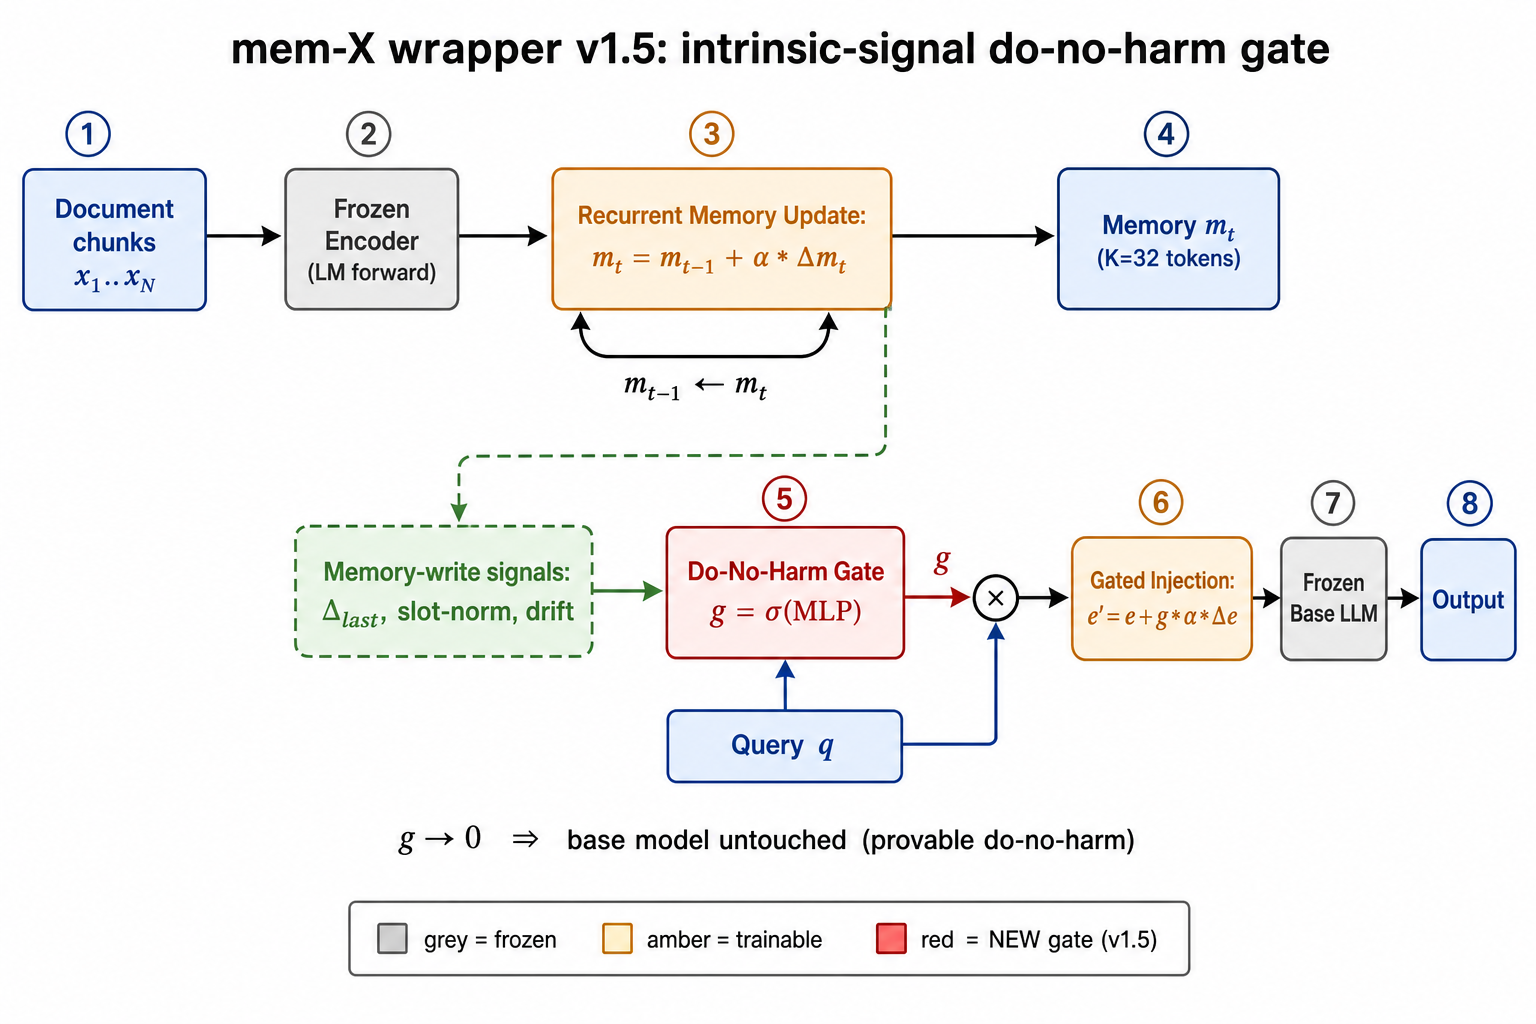
\includegraphics[width=0.86\linewidth]{../summary/2026-06-05/architecture-v1.5.png}
  \end{center}
  \vspace{-0.6em}
  \footnotesize Recurrent memory (carried from v0) $+$ a \textbf{do-no-harm gate} $g$: $e'=e+g\,\alpha\Delta e$, with $g{\to}0\Rightarrow$ the base is \emph{untouched}.
  $\rightarrow$ diagram source \texttt{summary/2026-06-05/architecture-v1.5.tex}; v0$\to$v1.5 diff in \texttt{summary/2026-06-05/v1.5-glossary.md}.
\end{frame}

\begin{frame}{The bet --- why this should work}
  \begin{itemize}
    \item \textbf{Hypothesis:} whether the wrapper will help is \emph{readable from the model's own forward pass} --- specifically from how much it \textbf{wrote into memory} ($\|\Delta m\|$, slot norms, drift).
    \item If true, a tiny gate on those signals can decide \textbf{per input} whether to open the wrapper or fall back to the base.
    \item \textbf{Crucial requirement:} those signals must be \emph{the same across model families} --- otherwise we'd re-tune per model and it's not deployable.
  \end{itemize}
  \vspace{0.6em}
  \footnotesize $\rightarrow$ candidate signals \& screen: \texttt{v1.5-metric-candidates-2026-06-04.md}; setting \texttt{P08-S6}.
\end{frame}

\begin{frame}{Result 1 --- \emph{where} it helps (expected vs.\ real)}
  \begin{columns}
    \begin{column}{0.55\linewidth}
      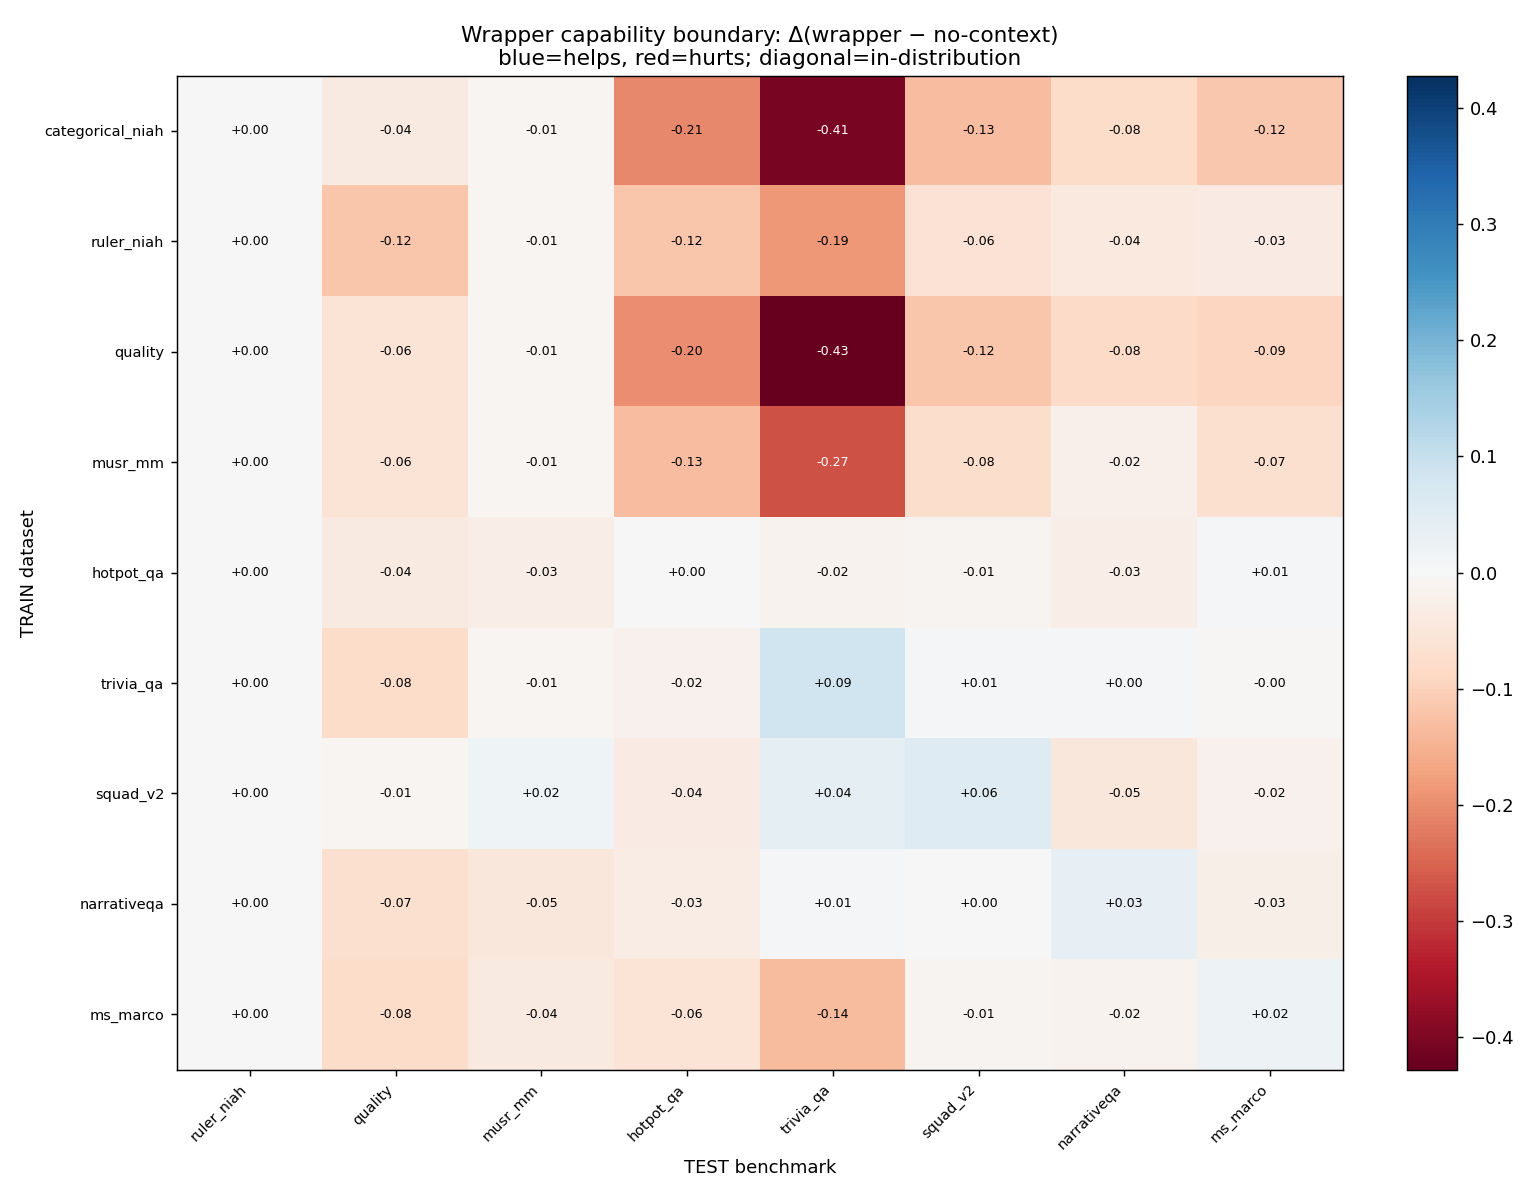
\includegraphics[width=\linewidth]{../raw/grids-xmodel-2026-06-05/transfer_heatmap.png}
    \end{column}
    \begin{column}{0.43\linewidth}
      \small
      \textbf{Expected:} helps where trained, decays as test drifts from train.\\[0.6em]
      \textbf{Real (72 train$\times$test cells):}
      \begin{itemize}\footnotesize
        \item \textbf{in-distribution: it helps} (QA $+2$ to $+9$ pt).
        \item competence is \textbf{distribution-bound}: gain $\to$ harm already at the same-task line.
      \end{itemize}
      \vspace{0.3em}\footnotesize $\rightarrow$ \texttt{P08-S7}, matrix \texttt{\S8}.
    \end{column}
  \end{columns}
\end{frame}

\begin{frame}{Result 2 --- \emph{deploy it safely} (expected vs.\ real)}
  \small
  \textbf{Expected:} one gate keeps the in-dist gains, avoids the OOD harm, and works on a new base model unchanged.
  \vspace{0.4em}
  \begin{block}{Real}
  \begin{itemize}
    \item \textbf{do-no-harm holds}: gated $\ge$ base on \textbf{32/35} cases.
    \item \textbf{model-agnostic}: the gate signal (\texttt{delta\_last}) predicts usefulness on an \textbf{unseen} family at AUROC \textbf{0.71} (leave-one-model-out, 7 families).
    \item \textbf{which signal generalizes:} memory-write dynamics (yes) vs.\ logit-lens confidence (no --- model-specific).
  \end{itemize}
  \end{block}
  \footnotesize $\rightarrow$ \texttt{P08-S6}/\texttt{P08-S8}, matrix \texttt{\S2b}/\texttt{\S7}; soft-gate that \emph{failed} (and why) $=$ \texttt{v1.5-gate-sweep-2026-06-05.md}.
\end{frame}

\begin{frame}{So what + honest scope + next}
  \textbf{Takeaway:} a frozen-base memory module becomes \textbf{safely deployable} --- it captures gains where it's competent and is provably harmless elsewhere, using one \emph{model-general} intrinsic signal.
  \vspace{0.6em}
  \begin{itemize}\small
    \item \textbf{Honest scope:} in-dist gains are \emph{modest \& dataset-dependent} (QA yes, multiple-choice no); the headline value is \textbf{safe, modular memory}, not SOTA.
    \item \textbf{Next:} (1) \emph{locking experiment} --- one gate that opens in-dist \& closes OOD on the same wrappers; (2) significance (more seeds + CIs); (3) \emph{mix-train} (all datasets) --- does multi-task training widen the boundary?
  \end{itemize}
  \vspace{0.5em}
  \footnotesize $\rightarrow$ full ledger \& asset index: \texttt{mem-embedding/summary/matrix.md}; decode any term: \texttt{v1.5-glossary.md}.
\end{frame}
 from main.tex. Figures: ../figs, ../raw/grids-xmodel-2026-06-05.
%  Wiki/details: ../summary/2026-06-05/v1.5-glossary.md, ../settings/settings.md, ../summary/2026-06-04/v1.5-metric-candidates-2026-06-04.md,
%                ../v1.5-gate-sweep-2026-06-05.md.
% =============================================================
\section{v1.5 --- Safe, model-agnostic memory gate (2026-06-05)}

\begin{frame}{v1.5: can a learned memory module be deployed \emph{safely}?}
  \large
  \begin{itemize}
    \item A frozen base + a small learned \textbf{memory wrapper}.
    \item \textbf{The question:} can we get its gains \emph{where it works} and \emph{never lose points} where it doesn't?
  \end{itemize}
  \vspace{1em}
  \normalsize One-line answer: \textbf{yes} --- an intrinsic-signal gate makes the wrapper
  \emph{help in-distribution} and \emph{do no harm out-of-distribution}, and it
  \textbf{transfers across 7 model families with no tuning}.
  \vspace{1.2em}\\
  \footnotesize $\rightarrow$ every term/number on the next slides links out to a wiki page: \texttt{v1.5-glossary.md}.
\end{frame}

\begin{frame}{Why it matters}
  \begin{itemize}
    \item \textbf{Frozen base = a promise: don't regress.} A memory/adaptation module is only deployable if it can't quietly \emph{hurt} the model on inputs it wasn't built for.
    \item \textbf{Our v1 finding:} the memory wrapper is a \emph{narrow lossy compressor} --- it helps on some inputs and \textbf{actively hurts} on others (e.g.\ exact-answer QA). Negative transfer is the blocker.
    \item \textbf{So the real product isn't "a better wrapper"} --- it's \textbf{knowing when to use it}, automatically, on any base model.
  \end{itemize}
  \vspace{0.8em}
  \footnotesize $\rightarrow$ v1 characterization (3-regime law): \texttt{v1-results-2026-06-03.md}.
\end{frame}

\begin{frame}{What we do (architecture)}
  \begin{center}
    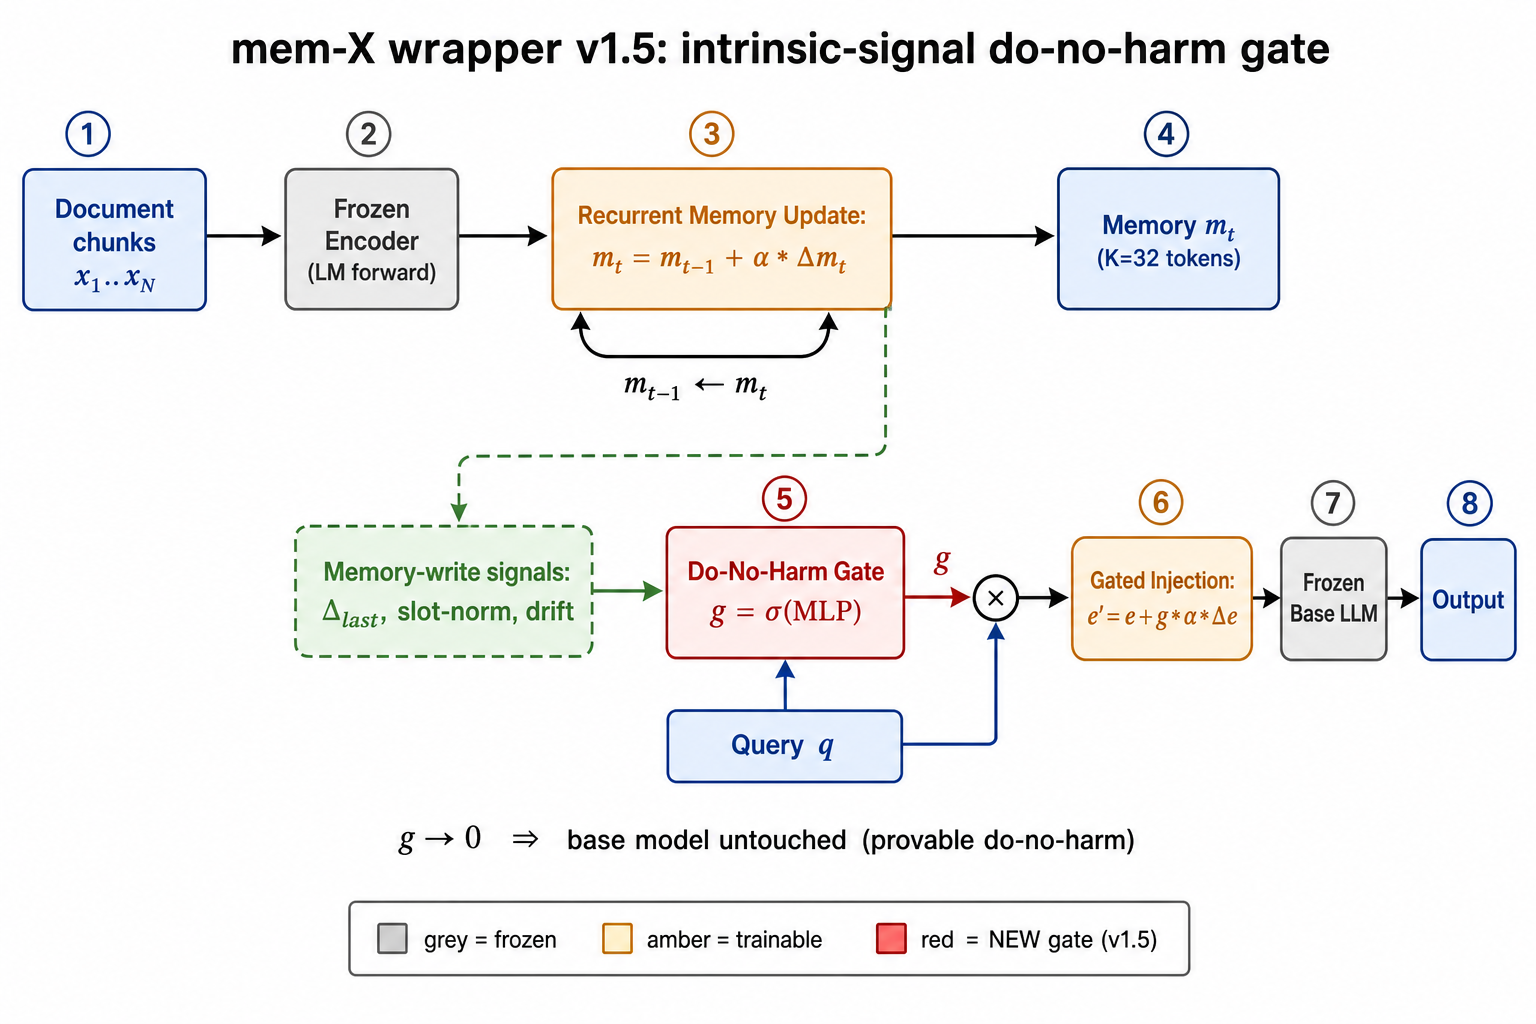
\includegraphics[width=0.86\linewidth]{../summary/2026-06-05/architecture-v1.5.png}
  \end{center}
  \vspace{-0.6em}
  \footnotesize Recurrent memory (carried from v0) $+$ a \textbf{do-no-harm gate} $g$: $e'=e+g\,\alpha\Delta e$, with $g{\to}0\Rightarrow$ the base is \emph{untouched}.
  $\rightarrow$ diagram source \texttt{summary/2026-06-05/architecture-v1.5.tex}; v0$\to$v1.5 diff in \texttt{summary/2026-06-05/v1.5-glossary.md}.
\end{frame}

\begin{frame}{The bet --- why this should work}
  \begin{itemize}
    \item \textbf{Hypothesis:} whether the wrapper will help is \emph{readable from the model's own forward pass} --- specifically from how much it \textbf{wrote into memory} ($\|\Delta m\|$, slot norms, drift).
    \item If true, a tiny gate on those signals can decide \textbf{per input} whether to open the wrapper or fall back to the base.
    \item \textbf{Crucial requirement:} those signals must be \emph{the same across model families} --- otherwise we'd re-tune per model and it's not deployable.
  \end{itemize}
  \vspace{0.6em}
  \footnotesize $\rightarrow$ candidate signals \& screen: \texttt{v1.5-metric-candidates-2026-06-04.md}; setting \texttt{P08-S6}.
\end{frame}

\begin{frame}{Result 1 --- \emph{where} it helps (expected vs.\ real)}
  \begin{columns}
    \begin{column}{0.55\linewidth}
      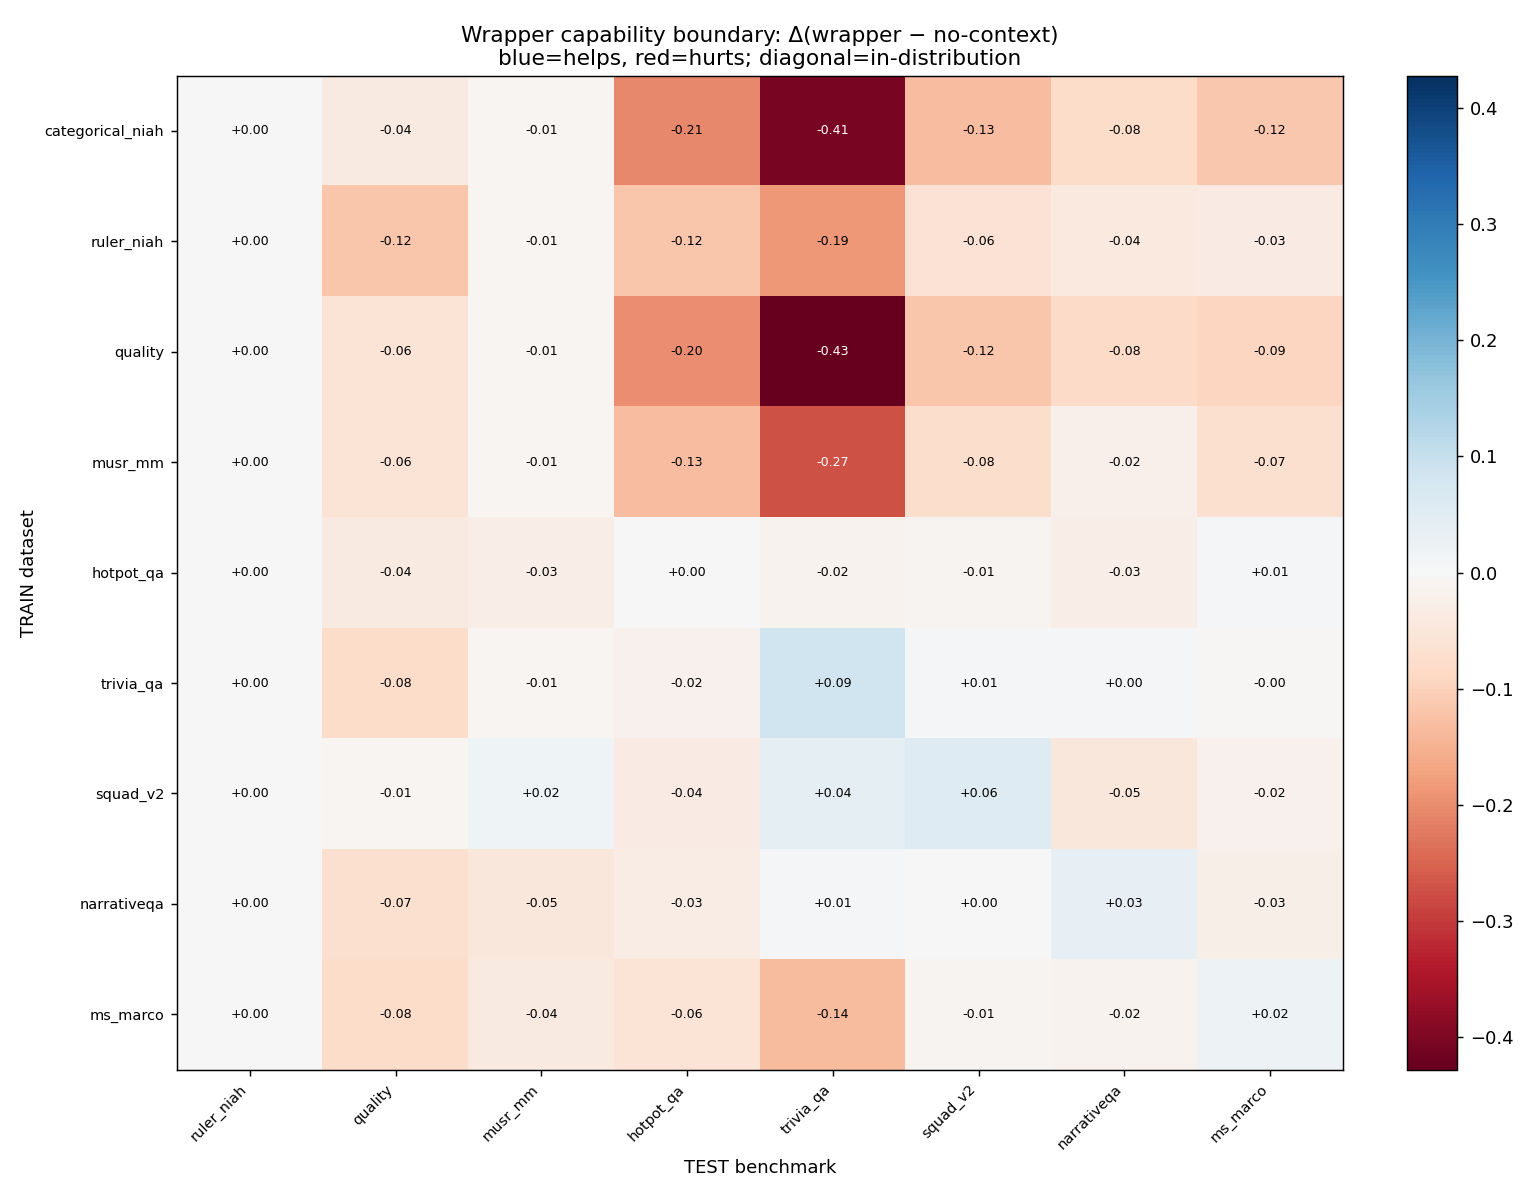
\includegraphics[width=\linewidth]{../raw/grids-xmodel-2026-06-05/transfer_heatmap.png}
    \end{column}
    \begin{column}{0.43\linewidth}
      \small
      \textbf{Expected:} helps where trained, decays as test drifts from train.\\[0.6em]
      \textbf{Real (72 train$\times$test cells):}
      \begin{itemize}\footnotesize
        \item \textbf{in-distribution: it helps} (QA $+2$ to $+9$ pt).
        \item competence is \textbf{distribution-bound}: gain $\to$ harm already at the same-task line.
      \end{itemize}
      \vspace{0.3em}\footnotesize $\rightarrow$ \texttt{P08-S7}, matrix \texttt{\S8}.
    \end{column}
  \end{columns}
\end{frame}

\begin{frame}{Result 2 --- \emph{deploy it safely} (expected vs.\ real)}
  \small
  \textbf{Expected:} one gate keeps the in-dist gains, avoids the OOD harm, and works on a new base model unchanged.
  \vspace{0.4em}
  \begin{block}{Real}
  \begin{itemize}
    \item \textbf{do-no-harm holds}: gated $\ge$ base on \textbf{32/35} cases.
    \item \textbf{model-agnostic}: the gate signal (\texttt{delta\_last}) predicts usefulness on an \textbf{unseen} family at AUROC \textbf{0.71} (leave-one-model-out, 7 families).
    \item \textbf{which signal generalizes:} memory-write dynamics (yes) vs.\ logit-lens confidence (no --- model-specific).
  \end{itemize}
  \end{block}
  \footnotesize $\rightarrow$ \texttt{P08-S6}/\texttt{P08-S8}, matrix \texttt{\S2b}/\texttt{\S7}; soft-gate that \emph{failed} (and why) $=$ \texttt{v1.5-gate-sweep-2026-06-05.md}.
\end{frame}

\begin{frame}{So what + honest scope + next}
  \textbf{Takeaway:} a frozen-base memory module becomes \textbf{safely deployable} --- it captures gains where it's competent and is provably harmless elsewhere, using one \emph{model-general} intrinsic signal.
  \vspace{0.6em}
  \begin{itemize}\small
    \item \textbf{Honest scope:} in-dist gains are \emph{modest \& dataset-dependent} (QA yes, multiple-choice no); the headline value is \textbf{safe, modular memory}, not SOTA.
    \item \textbf{Next:} (1) \emph{locking experiment} --- one gate that opens in-dist \& closes OOD on the same wrappers; (2) significance (more seeds + CIs); (3) \emph{mix-train} (all datasets) --- does multi-task training widen the boundary?
  \end{itemize}
  \vspace{0.5em}
  \footnotesize $\rightarrow$ full ledger \& asset index: \texttt{mem-embedding/summary/matrix.md}; decode any term: \texttt{v1.5-glossary.md}.
\end{frame}
 from main.tex. Figures: ../figs, ../raw/grids-xmodel-2026-06-05.
%  Wiki/details: ../summary/2026-06-05/v1.5-glossary.md, ../settings/settings.md, ../summary/2026-06-04/v1.5-metric-candidates-2026-06-04.md,
%                ../v1.5-gate-sweep-2026-06-05.md.
% =============================================================
\section{v1.5 --- Safe, model-agnostic memory gate (2026-06-05)}

\begin{frame}{v1.5: can a learned memory module be deployed \emph{safely}?}
  \large
  \begin{itemize}
    \item A frozen base + a small learned \textbf{memory wrapper}.
    \item \textbf{The question:} can we get its gains \emph{where it works} and \emph{never lose points} where it doesn't?
  \end{itemize}
  \vspace{1em}
  \normalsize One-line answer: \textbf{yes} --- an intrinsic-signal gate makes the wrapper
  \emph{help in-distribution} and \emph{do no harm out-of-distribution}, and it
  \textbf{transfers across 7 model families with no tuning}.
  \vspace{1.2em}\\
  \footnotesize $\rightarrow$ every term/number on the next slides links out to a wiki page: \texttt{v1.5-glossary.md}.
\end{frame}

\begin{frame}{Why it matters}
  \begin{itemize}
    \item \textbf{Frozen base = a promise: don't regress.} A memory/adaptation module is only deployable if it can't quietly \emph{hurt} the model on inputs it wasn't built for.
    \item \textbf{Our v1 finding:} the memory wrapper is a \emph{narrow lossy compressor} --- it helps on some inputs and \textbf{actively hurts} on others (e.g.\ exact-answer QA). Negative transfer is the blocker.
    \item \textbf{So the real product isn't "a better wrapper"} --- it's \textbf{knowing when to use it}, automatically, on any base model.
  \end{itemize}
  \vspace{0.8em}
  \footnotesize $\rightarrow$ v1 characterization (3-regime law): \texttt{v1-results-2026-06-03.md}.
\end{frame}

\begin{frame}{What we do (architecture)}
  \begin{center}
    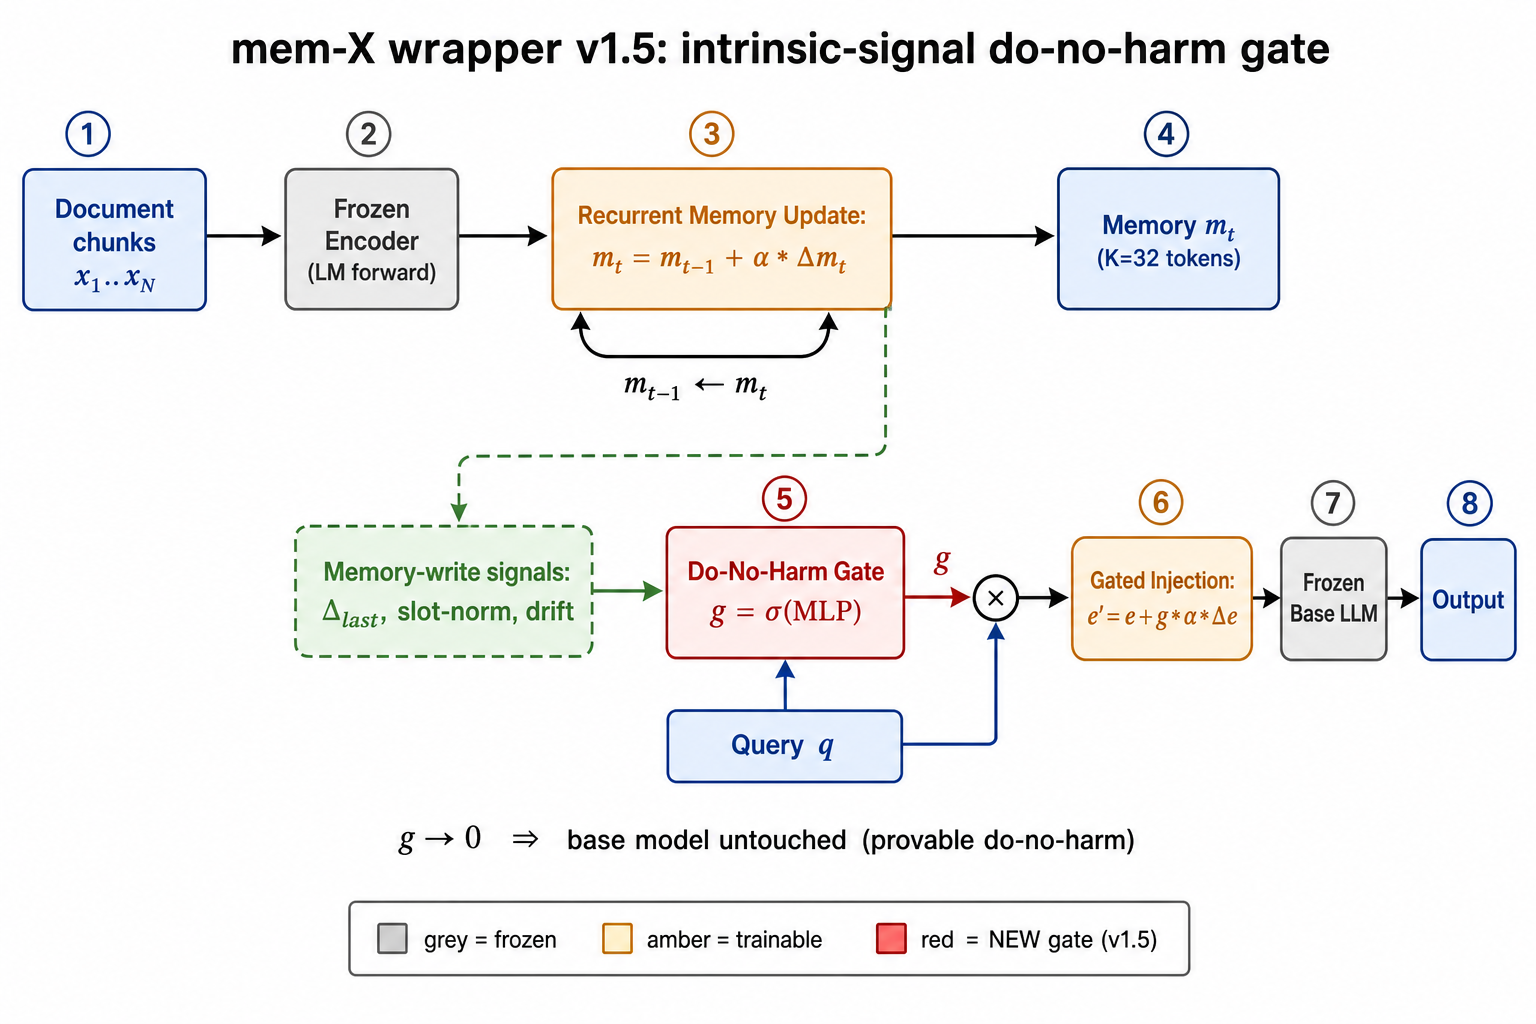
\includegraphics[width=0.86\linewidth]{../summary/2026-06-05/architecture-v1.5.png}
  \end{center}
  \vspace{-0.6em}
  \footnotesize Recurrent memory (carried from v0) $+$ a \textbf{do-no-harm gate} $g$: $e'=e+g\,\alpha\Delta e$, with $g{\to}0\Rightarrow$ the base is \emph{untouched}.
  $\rightarrow$ diagram source \texttt{summary/2026-06-05/architecture-v1.5.tex}; v0$\to$v1.5 diff in \texttt{summary/2026-06-05/v1.5-glossary.md}.
\end{frame}

\begin{frame}{The bet --- why this should work}
  \begin{itemize}
    \item \textbf{Hypothesis:} whether the wrapper will help is \emph{readable from the model's own forward pass} --- specifically from how much it \textbf{wrote into memory} ($\|\Delta m\|$, slot norms, drift).
    \item If true, a tiny gate on those signals can decide \textbf{per input} whether to open the wrapper or fall back to the base.
    \item \textbf{Crucial requirement:} those signals must be \emph{the same across model families} --- otherwise we'd re-tune per model and it's not deployable.
  \end{itemize}
  \vspace{0.6em}
  \footnotesize $\rightarrow$ candidate signals \& screen: \texttt{v1.5-metric-candidates-2026-06-04.md}; setting \texttt{P08-S6}.
\end{frame}

\begin{frame}{Result 1 --- \emph{where} it helps (expected vs.\ real)}
  \begin{columns}
    \begin{column}{0.55\linewidth}
      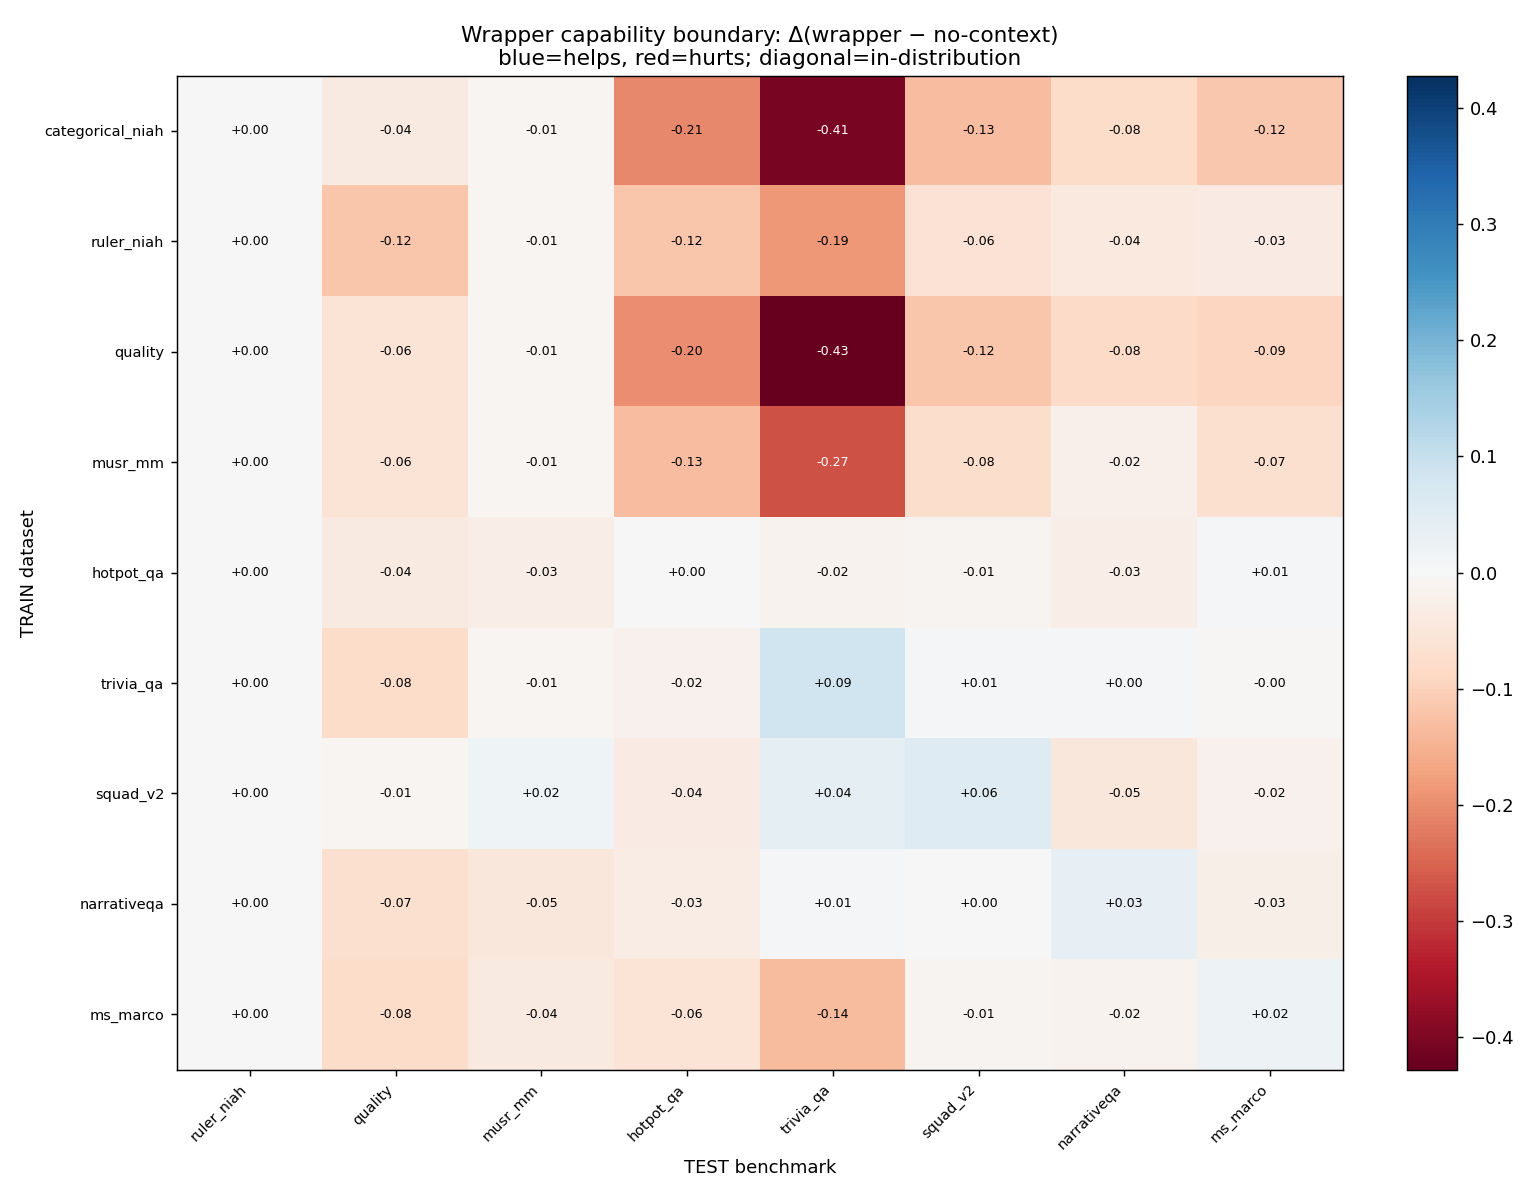
\includegraphics[width=\linewidth]{../raw/grids-xmodel-2026-06-05/transfer_heatmap.png}
    \end{column}
    \begin{column}{0.43\linewidth}
      \small
      \textbf{Expected:} helps where trained, decays as test drifts from train.\\[0.6em]
      \textbf{Real (72 train$\times$test cells):}
      \begin{itemize}\footnotesize
        \item \textbf{in-distribution: it helps} (QA $+2$ to $+9$ pt).
        \item competence is \textbf{distribution-bound}: gain $\to$ harm already at the same-task line.
      \end{itemize}
      \vspace{0.3em}\footnotesize $\rightarrow$ \texttt{P08-S7}, matrix \texttt{\S8}.
    \end{column}
  \end{columns}
\end{frame}

\begin{frame}{Result 2 --- \emph{deploy it safely} (expected vs.\ real)}
  \small
  \textbf{Expected:} one gate keeps the in-dist gains, avoids the OOD harm, and works on a new base model unchanged.
  \vspace{0.4em}
  \begin{block}{Real}
  \begin{itemize}
    \item \textbf{do-no-harm holds}: gated $\ge$ base on \textbf{32/35} cases.
    \item \textbf{model-agnostic}: the gate signal (\texttt{delta\_last}) predicts usefulness on an \textbf{unseen} family at AUROC \textbf{0.71} (leave-one-model-out, 7 families).
    \item \textbf{which signal generalizes:} memory-write dynamics (yes) vs.\ logit-lens confidence (no --- model-specific).
  \end{itemize}
  \end{block}
  \footnotesize $\rightarrow$ \texttt{P08-S6}/\texttt{P08-S8}, matrix \texttt{\S2b}/\texttt{\S7}; soft-gate that \emph{failed} (and why) $=$ \texttt{v1.5-gate-sweep-2026-06-05.md}.
\end{frame}

\begin{frame}{So what + honest scope + next}
  \textbf{Takeaway:} a frozen-base memory module becomes \textbf{safely deployable} --- it captures gains where it's competent and is provably harmless elsewhere, using one \emph{model-general} intrinsic signal.
  \vspace{0.6em}
  \begin{itemize}\small
    \item \textbf{Honest scope:} in-dist gains are \emph{modest \& dataset-dependent} (QA yes, multiple-choice no); the headline value is \textbf{safe, modular memory}, not SOTA.
    \item \textbf{Next:} (1) \emph{locking experiment} --- one gate that opens in-dist \& closes OOD on the same wrappers; (2) significance (more seeds + CIs); (3) \emph{mix-train} (all datasets) --- does multi-task training widen the boundary?
  \end{itemize}
  \vspace{0.5em}
  \footnotesize $\rightarrow$ full ledger \& asset index: \texttt{mem-embedding/summary/matrix.md}; decode any term: \texttt{v1.5-glossary.md}.
\end{frame}
 from main.tex. Figures: ../figs, ../raw/grids-xmodel-2026-06-05.
%  Wiki/details: ../summary/2026-06-05/v1.5-glossary.md, ../settings/settings.md, ../summary/2026-06-04/v1.5-metric-candidates-2026-06-04.md,
%                ../v1.5-gate-sweep-2026-06-05.md.
% =============================================================
\section{v1.5 --- Safe, model-agnostic memory gate (2026-06-05)}

\begin{frame}{v1.5: can a learned memory module be deployed \emph{safely}?}
  \large
  \begin{itemize}
    \item A frozen base + a small learned \textbf{memory wrapper}.
    \item \textbf{The question:} can we get its gains \emph{where it works} and \emph{never lose points} where it doesn't?
  \end{itemize}
  \vspace{1em}
  \normalsize One-line answer: \textbf{yes} --- an intrinsic-signal gate makes the wrapper
  \emph{help in-distribution} and \emph{do no harm out-of-distribution}, and it
  \textbf{transfers across 7 model families with no tuning}.
  \vspace{1.2em}\\
  \footnotesize $\rightarrow$ every term/number on the next slides links out to a wiki page: \texttt{v1.5-glossary.md}.
\end{frame}

\begin{frame}{Why it matters}
  \begin{itemize}
    \item \textbf{Frozen base = a promise: don't regress.} A memory/adaptation module is only deployable if it can't quietly \emph{hurt} the model on inputs it wasn't built for.
    \item \textbf{Our v1 finding:} the memory wrapper is a \emph{narrow lossy compressor} --- it helps on some inputs and \textbf{actively hurts} on others (e.g.\ exact-answer QA). Negative transfer is the blocker.
    \item \textbf{So the real product isn't "a better wrapper"} --- it's \textbf{knowing when to use it}, automatically, on any base model.
  \end{itemize}
  \vspace{0.8em}
  \footnotesize $\rightarrow$ v1 characterization (3-regime law): \texttt{v1-results-2026-06-03.md}.
\end{frame}

\begin{frame}{What we do (architecture)}
  \begin{center}
    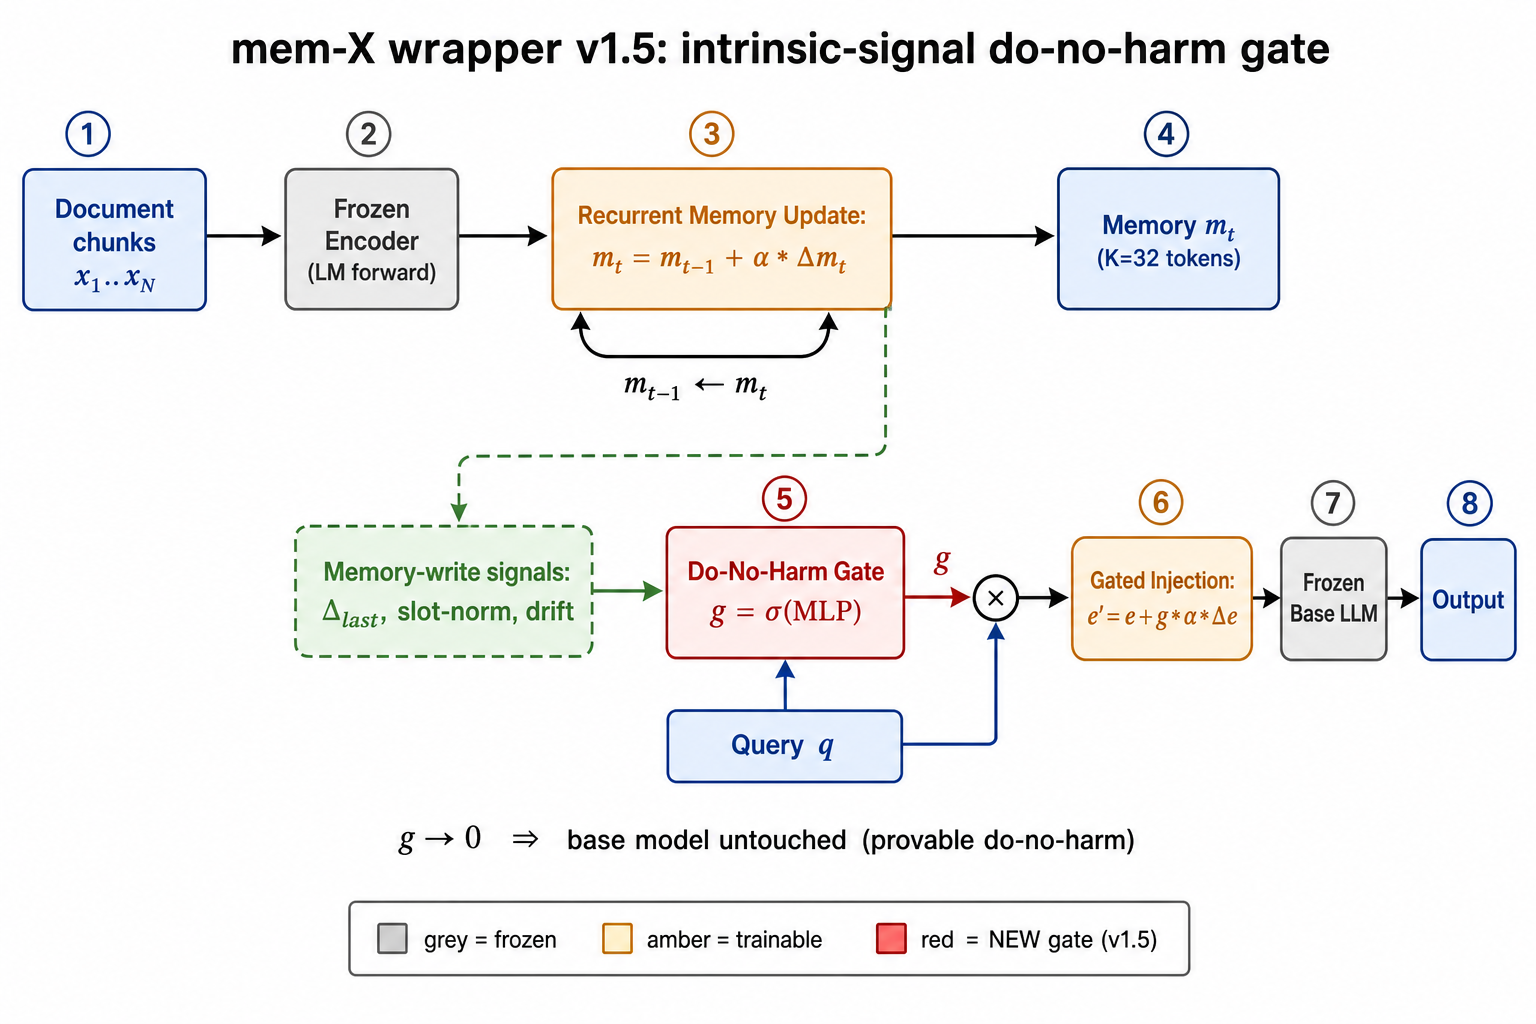
\includegraphics[width=0.86\linewidth]{../summary/2026-06-05/architecture-v1.5.png}
  \end{center}
  \vspace{-0.6em}
  \footnotesize Recurrent memory (carried from v0) $+$ a \textbf{do-no-harm gate} $g$: $e'=e+g\,\alpha\Delta e$, with $g{\to}0\Rightarrow$ the base is \emph{untouched}.
  $\rightarrow$ diagram source \texttt{summary/2026-06-05/architecture-v1.5.tex}; v0$\to$v1.5 diff in \texttt{summary/2026-06-05/v1.5-glossary.md}.
\end{frame}

\begin{frame}{The bet --- why this should work}
  \begin{itemize}
    \item \textbf{Hypothesis:} whether the wrapper will help is \emph{readable from the model's own forward pass} --- specifically from how much it \textbf{wrote into memory} ($\|\Delta m\|$, slot norms, drift).
    \item If true, a tiny gate on those signals can decide \textbf{per input} whether to open the wrapper or fall back to the base.
    \item \textbf{Crucial requirement:} those signals must be \emph{the same across model families} --- otherwise we'd re-tune per model and it's not deployable.
  \end{itemize}
  \vspace{0.6em}
  \footnotesize $\rightarrow$ candidate signals \& screen: \texttt{v1.5-metric-candidates-2026-06-04.md}; setting \texttt{P08-S6}.
\end{frame}

\begin{frame}{Result 1 --- \emph{where} it helps (expected vs.\ real)}
  \begin{columns}
    \begin{column}{0.55\linewidth}
      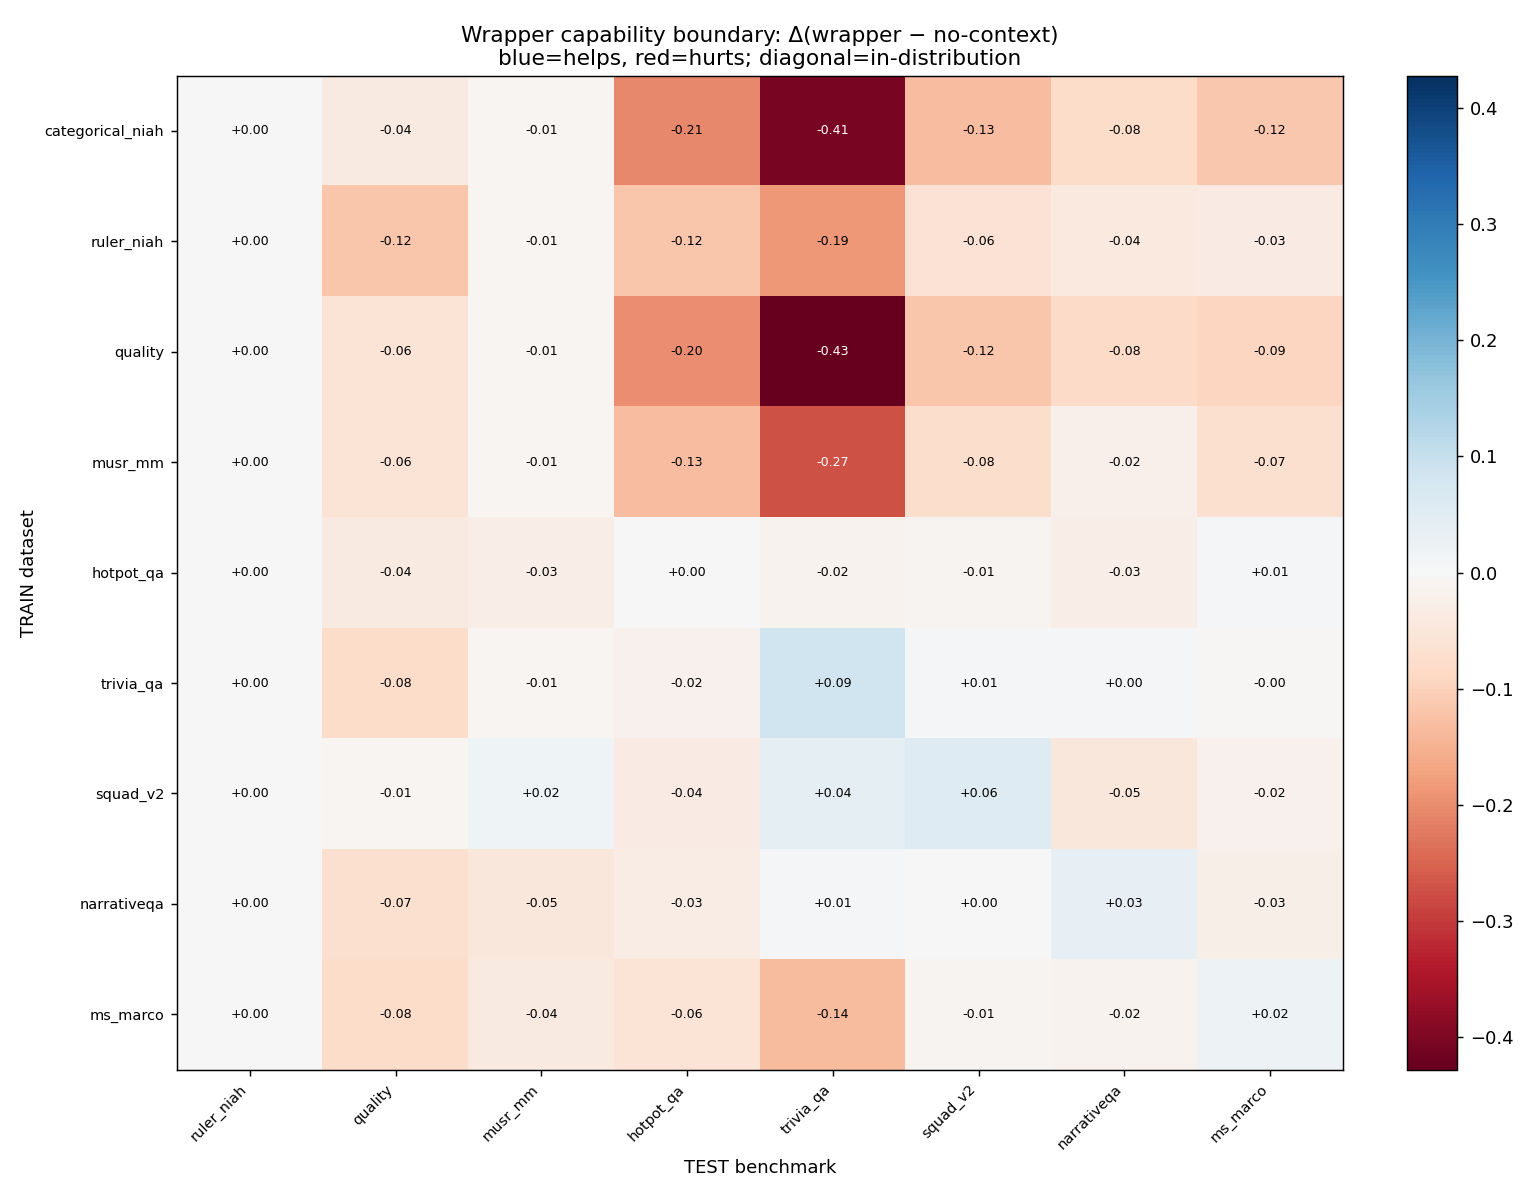
\includegraphics[width=\linewidth]{../raw/grids-xmodel-2026-06-05/transfer_heatmap.png}
    \end{column}
    \begin{column}{0.43\linewidth}
      \small
      \textbf{Expected:} helps where trained, decays as test drifts from train.\\[0.6em]
      \textbf{Real (72 train$\times$test cells):}
      \begin{itemize}\footnotesize
        \item \textbf{in-distribution: it helps} (QA $+2$ to $+9$ pt).
        \item competence is \textbf{distribution-bound}: gain $\to$ harm already at the same-task line.
      \end{itemize}
      \vspace{0.3em}\footnotesize $\rightarrow$ \texttt{P08-S7}, matrix \texttt{\S8}.
    \end{column}
  \end{columns}
\end{frame}

\begin{frame}{Result 2 --- \emph{deploy it safely} (expected vs.\ real)}
  \small
  \textbf{Expected:} one gate keeps the in-dist gains, avoids the OOD harm, and works on a new base model unchanged.
  \vspace{0.4em}
  \begin{block}{Real}
  \begin{itemize}
    \item \textbf{do-no-harm holds}: gated $\ge$ base on \textbf{32/35} cases.
    \item \textbf{model-agnostic}: the gate signal (\texttt{delta\_last}) predicts usefulness on an \textbf{unseen} family at AUROC \textbf{0.71} (leave-one-model-out, 7 families).
    \item \textbf{which signal generalizes:} memory-write dynamics (yes) vs.\ logit-lens confidence (no --- model-specific).
  \end{itemize}
  \end{block}
  \footnotesize $\rightarrow$ \texttt{P08-S6}/\texttt{P08-S8}, matrix \texttt{\S2b}/\texttt{\S7}; soft-gate that \emph{failed} (and why) $=$ \texttt{v1.5-gate-sweep-2026-06-05.md}.
\end{frame}

\begin{frame}{So what + honest scope + next}
  \textbf{Takeaway:} a frozen-base memory module becomes \textbf{safely deployable} --- it captures gains where it's competent and is provably harmless elsewhere, using one \emph{model-general} intrinsic signal.
  \vspace{0.6em}
  \begin{itemize}\small
    \item \textbf{Honest scope:} in-dist gains are \emph{modest \& dataset-dependent} (QA yes, multiple-choice no); the headline value is \textbf{safe, modular memory}, not SOTA.
    \item \textbf{Next:} (1) \emph{locking experiment} --- one gate that opens in-dist \& closes OOD on the same wrappers; (2) significance (more seeds + CIs); (3) \emph{mix-train} (all datasets) --- does multi-task training widen the boundary?
  \end{itemize}
  \vspace{0.5em}
  \footnotesize $\rightarrow$ full ledger \& asset index: \texttt{mem-embedding/summary/matrix.md}; decode any term: \texttt{v1.5-glossary.md}.
\end{frame}
